\begin{frame}
    \frametitle{Multilayer network}
    \begin{columns}
        \begin{column}{0.4\textwidth}
            \begin{definizione}
                Una \alert{multilayer network} è formata da un insieme di grafi
                detti \alert{layer} ed un insieme di \alert{inter-connessioni} 
                tra nodi appartenenti a layer differenti

            \end{definizione}
            % \pause
            \begin{exampleblock}{Alcuni esempi}
                \begin{enumerate}
                    \item Profili online in diversi social network
                    \item Stazioni di reti dei trasporti differenti
                \end{enumerate}
            \end{exampleblock}
        \end{column}
        \begin{column}{0.4\textwidth}
            \begin{figure}
                \centering
                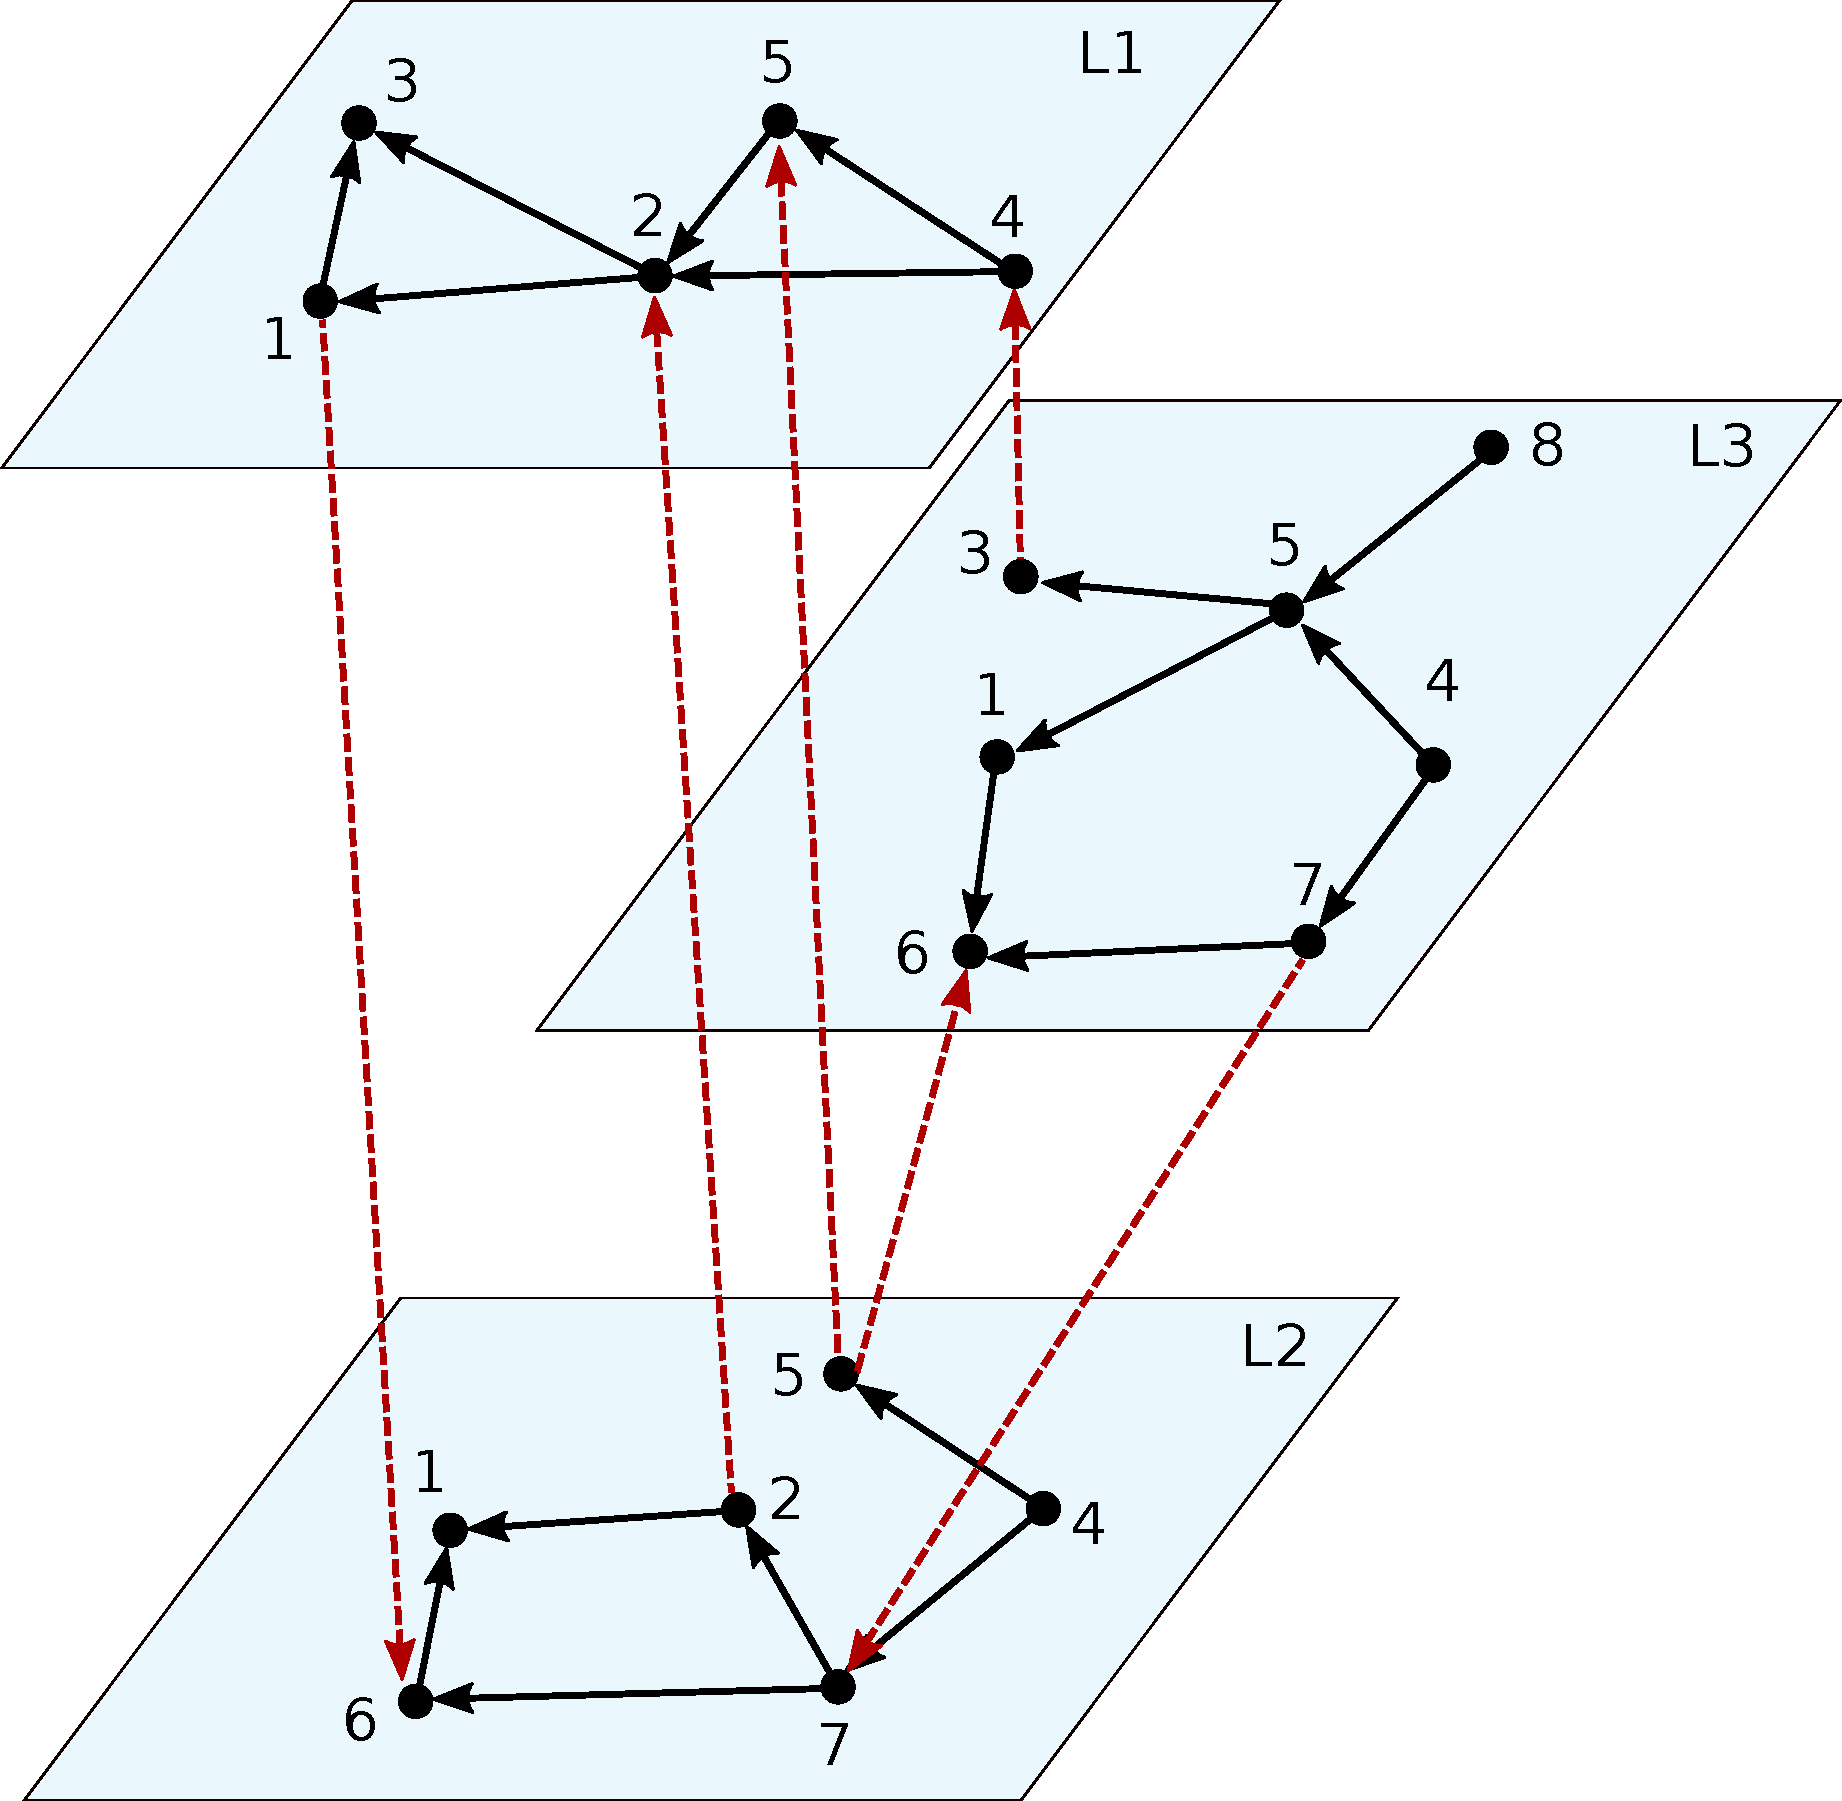
\includegraphics[width=\textwidth]{img/mlexample.pdf}
                % \caption{Grafo aggregato derivato dalla multilayer network rappresentata in Figura \ref{fig:mlexample}.}
                % \label{fig:graph}
            \end{figure}
        \end{column}
            
    \end{columns}
    

\end{frame}